\documentclass[]{mngt_deliverable}
\usepackage{graphicx}
\usepackage{hyperref}


%%%%%%%%%%%%%%%%%%%%%%
%%% Input project details
\def\studentname{Eva Darulov\'{a}}
\def\projecttitle{BON Software Model Consistency Checker for Eclipse}
\def\supervisorname{Dr. Joseph Kiniry}
\def\moderatorname{Dr. Barry Smith}


\begin{document}

\maketitle
%\tableofcontents\pdfbookmark[0]{Table of Contents}{toc}\newpage

%%%%%%%%%%%%%%%%%%%%%%
%%% Your Abstract here

\begin{abstract}
Modelling languages specifying a system independently from its 
implementation are particularly useful during analysis and design stages
of a system. An implementation-specific formal language translates those 
requirements directly into code, annotations and possibly assertions. 
Both approaches have their advantages and should ideally be used hand 
in hand. In practice however, mostly due to lack of tool support, the 
model of a project will not be updated once a formal specification is 
in place, thus rendering it useless. This project interlinks the BON and
JML modelling languages by creating a mapping between their structure 
and assertion features and by providing tool support for consistency 
checking. 
\end{abstract}
\newpage
\chapter{Introduction}
Business Object Notation (BON) has been developed for designing and analysing object-oriented programs. It is designed to enable a seamless and reversible development process as well as software contracting. It provides a textual, graphical and an informal representation of the system to be developed. Thus it can close the communication gap between technical and non-technical people (e.g. programmer and project manager) involved in the design and implementation of software.

The Java Modeling Language (JML) is a formal specification language for Java. It follows the Java syntax closely and its annotations are inserted directly into code. By doing so, it is easy for developers to learn and convenient to apply. It employs the design by contract approach by specifying preconditions, postconditions and invariants. With its extensive tool support it is greatly suitable for development of commercial software.

To make the most of a software model it has to be used throughout the development process, not just for the initial draft. For example, it can be used to update high-level manager on possible changes in the implementation without confusing them with technical details. This can only be achieved when the model is always up-to-date during whole of the development process. This project aims to provide such synchronisation by checking the consistency between a BON model and the corresponding Java source code with JML annotations.

\chapter{Project Management}
The following sections give a brief outline of the realization of the project.

\section{Tasks}
The detailed project time plan from December to the beginning of May is given in Figure 1.1. The tasks are divided into three main parts: Research, Implementation and Documentation. It is aimed that all background research will be completed by February. The implementation of the fundamental functionality is phased from December to mid March, since the individual parts depend on each other. The presentation, such as the implementation of the plugin and the GUI can be developed in parallel and are planned for January until April. These also include optional features, which, if delays should occur, will be abandoned. Finally, the documentation will be written towards the end of the project in March and April. This includes the final report as well as the documentation of the actual application.
Testing and code maintenance are ongoing processes and are thus planned after each major task.
\section{Milestones}
The project's progress is measured on the following five milestones:
\begin{description}
\item[1 - Basic functionality] A basic implementation that can compare BON and Java source code. Simple output is communicated to the user.
\item[2 - Eclipse plugin] The basic functionality has been inserted into an Eclipse plugin, so that the application can be directly used from within Eclipse without need for a command-line. Results are also presented in Eclipse.
\item[3 - Graphical User Interface] A GUI is implemented which makes the use of the application comfortable and straightforward. If options can be selected, they will be selected here.
\item[4 - Advanced functionality] Advanced functionality is implemented that also includes consistency checking between BON logic constructs and JML.
\item[5 - Finished application] A fully working Eclipse plugin.
\end{description}

\begin{figure}[h]
\centering
	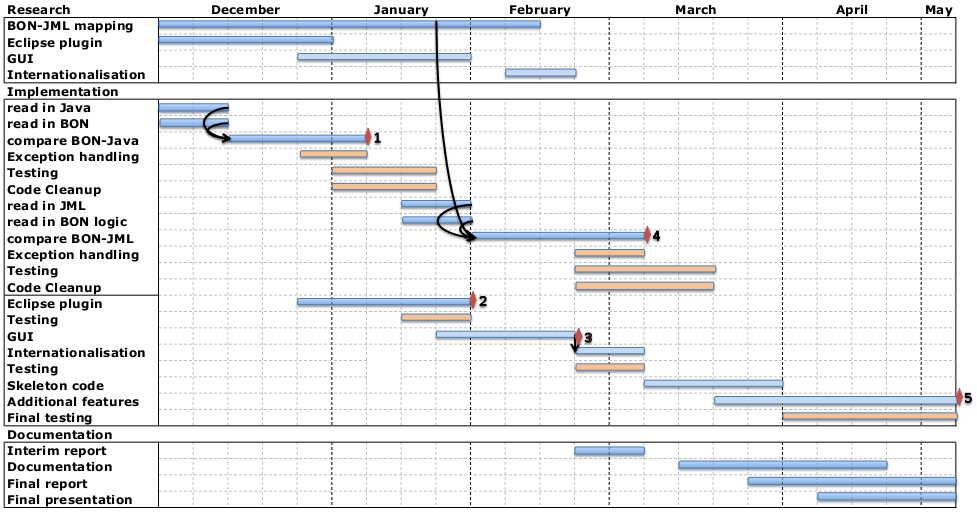
\includegraphics[width=1.0\textwidth]{ganttChart} 
	
\caption{\label{fig:logo} Tasks and Milestones. Priorities are denoted by the following colours: blue -mandatory, light blue - optional, orange - not in project description, but nevertheless graded. Milestones are indicated by red diamond shapes.}
\end{figure} 


\section{Risks}
The project is written in Java. Since this is a widely used programming language, no complications are expected. Furthermore, the project will use and so will rely on the open source projects OpenJML, BONc and Eclipse so that issues and incompatibilities may arise. However, OpenJML has already been tested on a small scale and deemed utilizable for this project. Eclipse plugins are being developed frequently, thus there exists are extensive community, so if problems should arise, there are resources for finding solutions. Finally, BONc is being developed by a PhD researcher in UCD, who can be contacted directly if trouble shooting should be needed.

\end{document}

\end{article}
